% !TEX program = lualatex

\documentclass{standalone}
\usepackage[utf8]{inputenc}

\usepackage{amsmath}
\usepackage{tikz-feynman}


\newcommand{\pbar}[1]{\overset{\textbf{\fontsize{4pt}{4pt}\selectfont(---)}}{#1}}

\begin{document}

%\feynmandiagram [vertical=a to b] {
%    i1 [particle=$\nu_\mu$]-- [fermion, momentum'=$p_\nu$] a -- [fermion, momentum'=$k_\mu$] f1 [particle=$\mu^-$],
%    a -- [boson, edge label'=$W^+$] b,
%    i2 [particle=$e^-$] -- [fermion, momentum'=$p_e$] b -- [fermion, momentum'=$k_e$] f2 [particle=$\nu_e$],
%};

%\feynmandiagram [horizontal=i1 to f1] {
%    i1 [particle=$\nu$] -- [fermion] v1 -- [fermion] f1 [particle=$\ell$],
%    i2 [blob] -- [fermion] v2 -- [fermion] q1 [blob],
%    v1 -- [boson, edge label=$W$] v2,
%    i2 -- [fermion] q1,
%    i2 -- [fermion] q1,    
%};

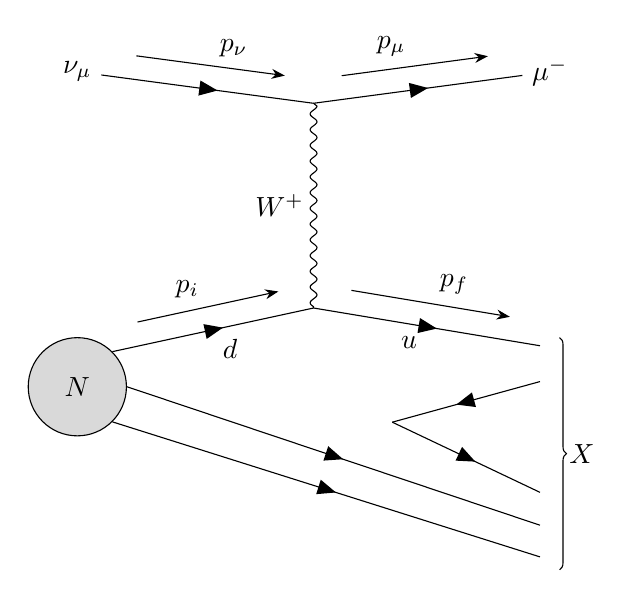
\begin{tikzpicture}
\begin{feynman}    
    % quark interaction point
    \vertex (interq) at (0,0);
    % lepton interaction point
    \vertex (interl) at (0, 2.6);
    % in/out leptons
    \vertex (il) at (-3, 3) {$\nu_\mu$};
    \vertex (ol) at (3, 3) {$\mu^-$};
    % input quarks (nucleus)
    \vertex (nuc) [shape=circle, draw, inner sep=0.3cm, fill=gray!30] at (-3, -1) {$N$};
    %\vertex (q1) at (-2, -0.5) {};
    %\vertex[below=0.4cm of q1] (q2) {};
    %\vertex[below=0.4cm of q2] (q3) {};
    % output quarks (shower)
    \vertex (x1) at (3, -0.5) {};
    \vertex[below=0.4cm of x1] (x2) {};
    \vertex[below=1.5cm of x2] (x3) {};
    \vertex (hadr) at ($(x2)!0.5!(x3) + (-2,0.2)$);
    \vertex[below=0.4cm of x3] (x4) {};
    \vertex[below=0.4cm of x4] (x5) {};
    
    
    \diagram*{
        % (q1) -- [fermion] (interq) -- [fermion] (x1),
        % (q2) -- [fermion] (x4),
        % (q3) -- [fermion] (x5),
        (nuc.north east) -- [fermion, edge label'=$d$, momentum=$p_i$] (interq) -- [fermion, edge label'=$u$, momentum=$p_f$] (x1),
        (nuc.east) -- [fermion] (x4),
        (nuc.south east) -- [fermion] (x5),
        (x2) -- [fermion] (hadr) -- [fermion] (x3),
        (interq) -- [boson, edge label=$W^+$] (interl),
        (il) -- [fermion, momentum=$p_\nu$] (interl) -- [fermion, momentum=$p_\mu$] (ol),
    };
    
    %\draw [decoration={brace}, decorate]  (q3.south west) -- (q1.north west) node [pos=0.5, left] {$N$};
    
    \draw [decoration={brace}, decorate]  (x1.north east) -- (x5.south east) node [pos=0.5, right] {$X$};
\end{feynman}
\end{tikzpicture}
\end{document}